% Drawing 142/06-4 -- folder 142, batch 06, archive page 105 (PDF page 106).
% Transcription: Quatrième figure. Cercles autour de $0$ et $1$, un chemin $a^\infty$ de $0$ vers $1$, le point $\infty$ isolé dans un petit cercle. Inscriptions $\Lambda^0_+ = (\Lambda^0_-)^{-1}$, $\Lambda'^1_- = (\Lambda'^1_+)^{-1}$. Légende : « 2 sommets, trois flèches, 0 relation » ; dessous : « 3 cas ».
% Kind: quiver on the sphere minus three points (small circles and paths). Method 2 (schematic redraw from the facsimile). Status: ok.
% Notes: Circles round 0 and 1 with the path a^infty from 0 to 1; infinity isolated in a small pencil circle; a pencil loop round the figure. Inscriptions Lambda^0_+ = (Lambda^0_-)^{-1}, Lambda'^1_- = (Lambda'^1_+)^{-1}; legends "2 sommets, trois fleches, 0 relation" and "3 cas".
% Coordinates: 1 unit = 1 mm = 1/100 of the crop width (bbox in page fractions: [0.5, 0.248, 0.884, 0.406]).
% Redrawn by Claude (claude-opus-5-5), issue #73, 2026-11-07; not checked by a human; not compiled (no TeX in the session).
% Rights: reproduces part of the work -- behind RENDER_TRANSCRIPTS, never published by itself.
\documentclass[tikz,border=3pt]{standalone}
\usepackage{amsmath,amssymb}
\usetikzlibrary{patterns,arrows.meta}
\tikzset{pencil/.style={black!45}, struck/.style={black!35}, mark/.style={circle,draw,inner sep=1.3pt}, pt/.style={circle,fill,inner sep=0.9pt}, opt/.style={circle,draw,fill=white,inner sep=1.1pt}}
\begin{document}
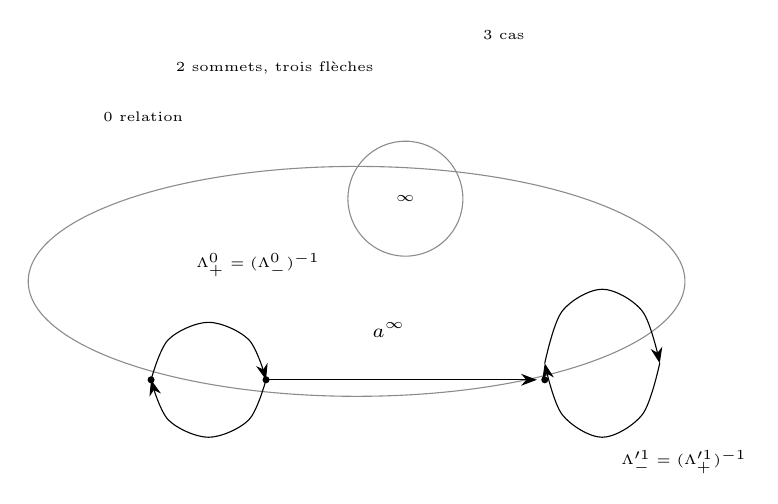
\begin{tikzpicture}[x=1mm,y=1mm,line cap=round,line join=round,font=\scriptsize]
\draw[pencil] (41.7,-31.3) ellipse[x radius=41.7, y radius=14.6];
\draw[pencil] (47.9,-20.8) circle[radius=7.3];
\node[inner sep=1pt] at (47.9,-20.8) {\tiny $\infty$};
\draw[-{Stealth[length=2mm]}] plot[smooth, tension=0.55] coordinates {(15.6,-43.8) (17.8,-38.7) (22.9,-36.5) (28,-38.7) (30.2,-43.8)};
\draw[-{Stealth[length=2mm]}] plot[smooth, tension=0.55] coordinates {(30.2,-43.8) (28,-48.9) (22.9,-51.1) (17.8,-48.9) (15.6,-43.8)};
\draw[-{Stealth[length=2mm]}] plot[smooth, tension=0.55] coordinates {(65.6,-41.7) (67.8,-35.1) (72.9,-32.3) (78,-35.1) (80.2,-41.7)};
\draw[-{Stealth[length=2mm]}] plot[smooth, tension=0.55] coordinates {(80.2,-41.7) (78,-48.2) (72.9,-51.1) (67.8,-48.2) (65.6,-41.7)};
\node[pt] at (15.6,-43.8) {};
\node[pt] at (30.2,-43.8) {};
\node[pt] at (65.6,-43.8) {};
\draw[-{Stealth[length=2mm]}] (30.2,-43.8) -- (64.6,-43.8);
\node[inner sep=1pt] at (45.8,-37.5) {\scriptsize $a^\infty$};
\node[inner sep=1pt] at (29.2,-29.2) {\tiny $\Lambda^0_+=(\Lambda^0_-)^{-1}$};
\node[inner sep=1pt] at (83.3,-54.2) {\tiny $\Lambda'^1_-=(\Lambda'^1_+)^{-1}$};
\node[inner sep=1pt] at (31.3,-4.2) {\tiny 2 sommets, trois fl\`eches};
\node[inner sep=1pt] at (14.6,-10.4) {\tiny 0 relation};
\node[inner sep=1pt] at (60.4,-0) {\tiny 3 cas};
\end{tikzpicture}
\end{document}
